% Name: Ripple-carry adder
% Description: Four full adders chained into a 4-bit adder: each takes one bit of A and B, and its carry out ripples into the next adder on the left.
% Tags: ripple-carry adder, full adder, binary addition, arithmetic circuit

\usetikzlibrary{arrows.meta}

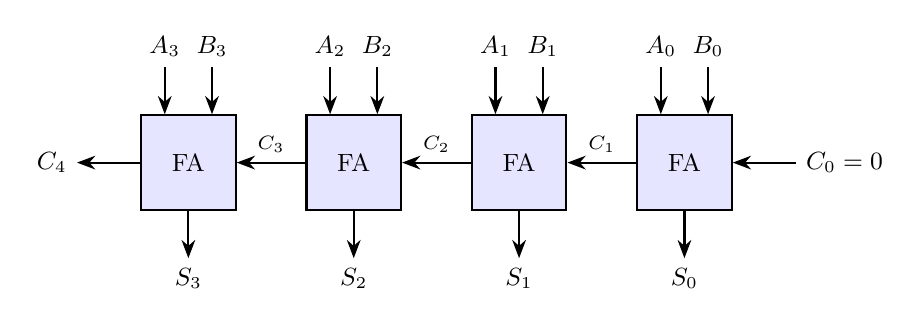
\begin{tikzpicture}[>={Stealth}, thick, every node/.style={font=\small},
    fa/.style={draw, fill=blue!10, minimum width=12mm, minimum height=12mm}]
  % Bit i sits at x = 6.3 - 2.1i, so the least significant bit is on the right
  \foreach \i in {0,...,3} {
    \pgfmathsetmacro\x{6.3 - 2.1*\i}
    \node[fa] (fa\i) at (\x,0) {FA};
    \draw[<-] ([xshift=-3mm]fa\i.north) -- ++(0,0.6) node[above] {$A_\i$};
    \draw[<-] ([xshift=3mm]fa\i.north) -- ++(0,0.6) node[above] {$B_\i$};
    \draw[->] (fa\i.south) -- ++(0,-0.6) node[below] {$S_\i$};
  }
  \foreach \i/\j in {0/1, 1/2, 2/3} \draw[->] (fa\i.west) -- node[above, font=\scriptsize] {$C_\j$} (fa\j.east);
  \draw[<-] (fa0.east) -- ++(0.8,0) node[right] {$C_0 = 0$};
  \draw[->] (fa3.west) -- ++(-0.8,0) node[left] {$C_4$};
\end{tikzpicture}
